
\section{Method}


\subsection{Data}

The image data used are captured by the earth observation satellite WorldView3
owned by DigitalGlobe. The WorldView3 satellite produces multiple categories of
imagery with varying degrees of resolution. The panchromatic images have
a resolution of 0.31 meter in contrast to  the multiband images have
a significantly lower resolution of
1.24 meter. The project uses pansharpened images, which combines the high
resolution panchromatic- and the low resolution multiband images to create
high resolution RGB images.

The content of the images contain regions of Bangalore, which is the capital
city of the indian state of Karnataka, located in south central India. The
population of the city is over ten million and is recognized as a mega city.
Banglore is known to have problems concerning informal settlements. According
to a report from 2012, there are 862 reported slums in the city


\begin{figure}
  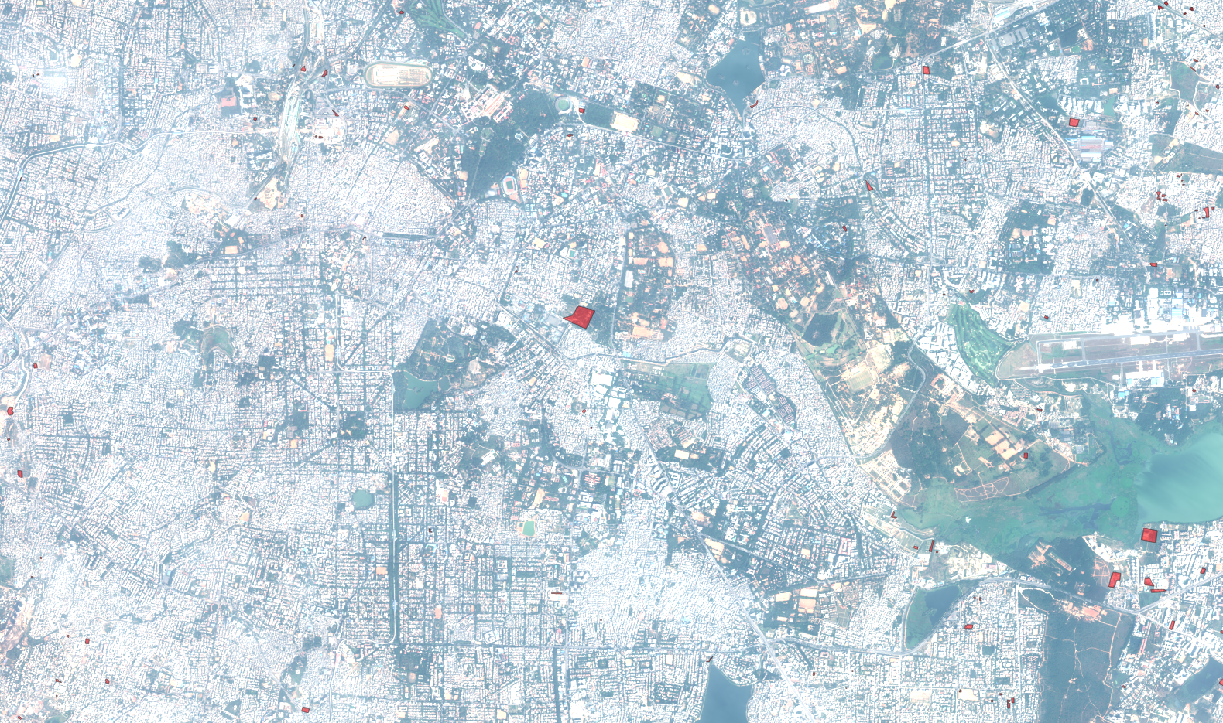
\includegraphics[width=\linewidth]{images/west-bangalore}
  \caption{A part of western Bangalore, the red patches indicate informal
  settlements}
  \label{fig:west-bangalore}
\end{figure}

\subsection{Challenges}
The distinction between formal and informal regions is often quite challenging,
in part due to the vagueness of borders between the regions. The border between
formal and informal regions often resembles more of a spectrum than a clear cut line.
Besides border difficulties, some areas are not designated as informal, while
still posessing characteristics of an informal region. This results in
a dataset with noise and inconsistency.  All in all, the binary classification
of a region encounters difficulties when applied in practice. 


Another challenge encountered in this field is the scarcity of informal
settlements.  Eventhough Banglore  has an abundance of informal settlements,
the fast majority of land is identified as formal area's. Figure
\ref{fig:west-bangalore} shows a part of western Bangalore where it is clear
that informal settlements are sparce and distributed throughout the city. As
a result, the dataset of formal and informal regions becomes quite skewed.
Furthermore, because everything that is not informal is automatically
considered formal, the formal regions have a large amount of variance of visual
properties.  To illustrate: lakes, forrests, and fields fall in the same
catagory as formal residential and industrial areas while the visual
characteristics are significantly different. The diverse content of the formal
set of visual characteristics might hinder the effectiveness of differentiating
between formal and informal regions. 

To reduce the skewedness between informal and formal, only subsections of Figure \ref{fig:west-bangalore} are
used where the proportion formal to informal is less one-sided. An example of
such a region is Figure \ref{fig:section_3}. A smaller difference in formal
informal ratio allows for a better understanding of the effectiveness of
various features. The features are assesed using these area's 

\begin{figure}
\centering
  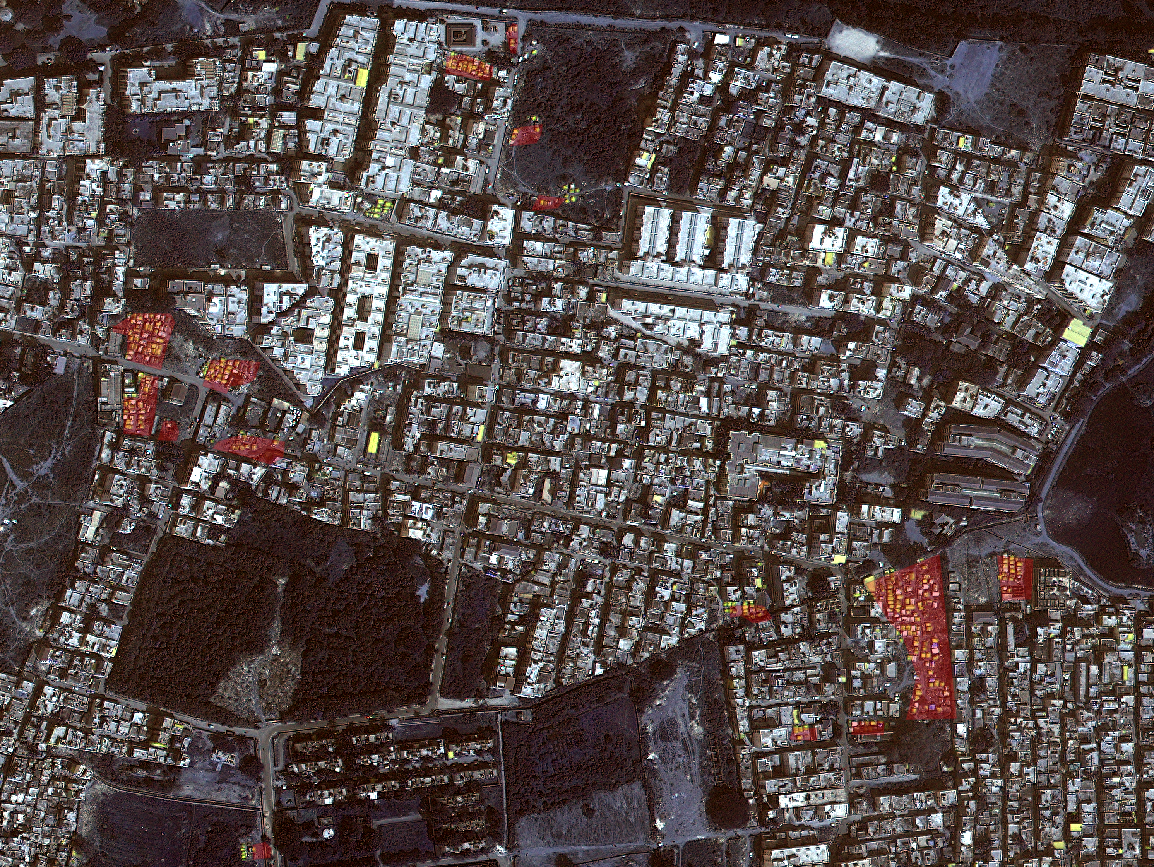
\includegraphics[width=\linewidth]{images/section_3}
  \caption{Dense informal area in Bangalore, the red patches indicate informal
  settlements}
  \label{fig:section_3}
\end{figure}


